\documentclass[10pt]{article}
\usepackage[margin=0.62in]{geometry}
\usepackage{amsmath,amssymb,enumitem,xcolor,tikz,fancyvrb,fontspec}
\usetikzlibrary{arrows.meta,positioning}
\pagestyle{empty}
\setlist{nosep,leftmargin=1.3em}
\definecolor{hi}{RGB}{130,25,35}
\newfontfamily\leanfont{DejaVu Sans}
\newenvironment{lean}{\Verbatim[fontsize=\scriptsize,frame=single,framesep=1.5mm,formatcom=\leanfont]}{\endVerbatim}
\newcommand{\high}{\textcolor{hi}{\textbf{Change}}}
\newcommand{\keep}{\textbf{Keep}}
\begin{document}
\begin{center}
{\Large\bfseries Upstream review: two periodicity APIs}\\[-1mm]
\small additive endomorphism geometric sums; finite-field Frobenius
\end{center}
\small

\section*{Verdict}
Both APIs are mathematically correct, small, and reusable. The Frobenius pair is essentially ready.
For the endomorphism pair, replace the bespoke induction by specialization of
\texttt{mul\_geom\_sum}; this removes \texttt{Mathlib.Tactic.Abel} and makes the intended API
relationship explicit. I would upstream the pairs separately.

\section*{1. Additive endomorphisms}
\subsection*{Use the ring theorem already imported --- \high}
The submitted proof re-proves the geometric identity by induction, although
\texttt{Mathlib.Algebra.Ring.GeomSum} supplies
\begin{lean}
mul_geom_sum phi n :
  (phi - 1) * (sum i in range n, phi ^ i) = phi ^ n - 1
\end{lean}
Evaluate this identity at \texttt{x}. The only coercion bridge needed is evaluation of the finite
sum; package evaluation as an additive hom and use root-level \texttt{map\_sum}:
\begin{lean}
let ev : AddMonoid.End A ->+ A :=
  { toFun := fun f => f x
    map_zero' := rfl
    map_add' := fun _ _ => rfl }
have hsum : ((sum i in range n, phi ^ i) : AddMonoid.End A) x =
    sum i in range n, (phi ^ i) x :=
  map_sum ev (fun i => phi ^ i) (range n)
have h := congrArg (fun f : AddMonoid.End A => f x)
  (mul_geom_sum phi n)
change phi ((sum i in range n, phi ^ i) x) -
  (sum i in range n, phi ^ i) x = (phi ^ n) x - x at h
rwa [hsum] at h
\end{lean}
This is shorter conceptually, avoids duplicated algebra, and needs no tactic import.

\subsection*{Simplify the fixed-point corollary --- \high}
The current proof converts equality to subtraction twice through nested \texttt{simpa}. Prefer the
visible one-line calculation:
\begin{lean}
rw [<- sub_eq_zero, apply_sum_pow_sub, hphi]
simp
\end{lean}
The submitted proof is valid; this is a readability change.

\subsection*{Placement and names --- \keep}
Do not add the geometric-sum dependency directly to the foundational
\texttt{Algebra.Group.Hom.End} file merely for two corollaries. A small file such as
\texttt{Algebra/Group/EndomorphismGeomSum.lean} is the clean dependency direction. The namespace and
hypothesis \texttt{[AddCommGroup A]} are right. The existing names are discoverable from
\texttt{AddMonoid.End}; an alternative aligned more tightly with the source lemma is
\texttt{apply\_mul\_geom\_sum}, but renaming is not required.

\begin{center}
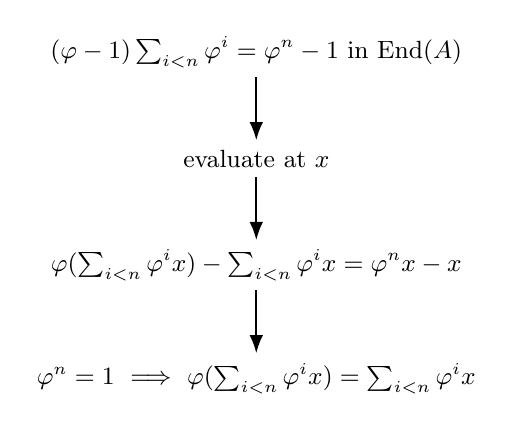
\begin{tikzpicture}[>=Latex,node distance=8mm and 13mm,every node/.style={font=\small}]
\node (ring) {$ (\varphi-1)\sum_{i<n}\varphi^i=\varphi^n-1$ in $\operatorname{End}(A)$};
\node[below=of ring] (eval) {evaluate at $x$};
\node[below=of eval] (point) {$\varphi(\sum_{i<n}\varphi^i x)-\sum_{i<n}\varphi^i x=\varphi^n x-x$};
\node[below=of point] (fixed) {$\varphi^n=1\ \Longrightarrow\ \varphi(\sum_{i<n}\varphi^i x)=\sum_{i<n}\varphi^i x$};
\draw[->,thick] (ring)--(eval); \draw[->,thick] (eval)--(point); \draw[->,thick] (point)--(fixed);
\end{tikzpicture}
\end{center}

\newpage
\section*{2. Finite-field Frobenius}
\subsection*{The abstraction is exactly right --- \keep}
\begin{lean}
theorem frobenius_pow_eq_pow_mod
    (hcard : Fintype.card K = p ^ n) (m : Nat) :
    frobenius K p ^ m = frobenius K p ^ (m % n) :=
  pow_eq_pow_mod m (FiniteField.frobenius_pow hcard)
\end{lean}
This is the natural generic corollary of \texttt{FiniteField.frobenius\_pow}. Keep both the
endomorphism equality and pointwise theorem: they serve different rewrite contexts. The proof of the
pointwise theorem is already minimal and clear.

\subsection*{Drop the redundant import --- \high}
\begin{lean}
import Mathlib.FieldTheory.Finite.Basic
import Mathlib.GroupTheory.OrderOfElement
\end{lean}
The second import is unnecessary: \texttt{pow\_eq\_pow\_mod},
\texttt{FiniteField.frobenius\_pow}, and \texttt{iterateFrobenius\_eq\_pow} are all available from
\texttt{Mathlib.FieldTheory.Finite.Basic} in the audited Mathlib version. Keep only the first import.
If declarations are inserted directly after \texttt{frobenius\_pow} in that same file, no new import
is needed at all.

\subsection*{No positivity hypothesis is needed --- \keep}
Do not add \texttt{0 < n}. The generic theorem handles \texttt{n = 0}, and the cardinality premise is
already incompatible with a nontrivial finite field having cardinality $p^0=1$. The current statement
is minimal and faithful.

\subsection*{Documentation and naming --- minor}
The module text says ``extension degree.'' The formal input is only a cardinality equality, so
``exponent in the cardinality presentation'' is maximally literal; ``extension degree'' is standard
and acceptable in this finite-field context. \texttt{iterateFrobenius\_mod} matches existing concise
Frobenius naming. Add \texttt{eq} only if a maintainer requests strict equality-name style.

\begin{center}
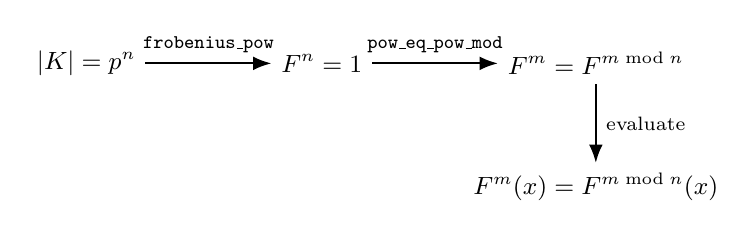
\begin{tikzpicture}[>=Latex,node distance=10mm and 16mm,every node/.style={font=\small}]
\node (card) {$|K|=p^n$};
\node[right=of card] (period) {$F^n=1$};
\node[right=of period] (reduce) {$F^m=F^{m\bmod n}$};
\node[below=of reduce] (point) {$F^m(x)=F^{m\bmod n}(x)$};
\draw[->,thick] (card)--node[above]{\scriptsize\texttt{frobenius\_pow}}(period);
\draw[->,thick] (period)--node[above]{\scriptsize\texttt{pow\_eq\_pow\_mod}}(reduce);
\draw[->,thick] (reduce)--node[right]{\scriptsize evaluate}(point);
\end{tikzpicture}
\end{center}

\section*{Suggested PR split}
\begin{enumerate}
\item Endomorphism PR: new geometric-sum companion file; ring-level specialization; no
\texttt{Tactic.Abel}.
\item Finite-field PR: place both lemmas immediately after \texttt{FiniteField.frobenius\_pow}; no
extra import.
\end{enumerate}

\section*{Verification}
All four declarations were compiled together against the pinned Mathlib version. The endomorphism
proof was also compiled in its recommended ring-theorem form. No \texttt{sorry} is used.
\end{document}
